\documentclass[border={10pt 10pt 10pt 10pt}]{standalone}

\usepackage{siunitx}
\usepackage{ifthen}
\usepackage{tikz}
\usetikzlibrary{positioning,shapes,shadows,arrows}

\newlength{\hp}
\newlength{\hs}
\newlength{\vs}
\setlength{\hp}{3pt}
\setlength{\hs}{0.5cm}
\setlength{\vs}{0.8cm}
% \renewcommand{\baselinestretch}{.8}

\newcommand{\hsep}{\\[\hp]\hrule\vspace{\hp}}
\newcommand{\hhsep}{\\[\hp]\hrule\vspace{1pt}\hrule\vspace{2\hp}}


\newcommand{\subone}[1]{\number\numexpr#1-1\relax}

\newcommand{\getnode}[3]{
    \ifthenelse{\not\equal{#1}{0}}{
        \ifthenelse{\equal{#1}{1}}{
            \node(Q#1)[block, above=\hs of Q\subone{#1}]{#2};
        }{
            \ifthenelse{\equal{#1}{9}}{
                \node(Q#1)[block, below=\hs of Q\subone{#1}]{#2};
            }{
                \ifthenelse{#1>9}{
                    \node(Q#1)[block, left=\vs of Q\subone{#1}]{#2};
                }{
                    \node(Q#1)[block, right=\vs of Q\subone{#1}]{#2};
                }
            }

        }
    }{
        \node(Q#1)[block]{#2};
    }
}

\newcommand{\qubit}[5]{
    \getnode{#1}{$Q_{#1}$\hsep #2\\#3\\#4\\#5}
}


\newcommand{\displaycxerror}[1]{$#1$}

\begin{document}
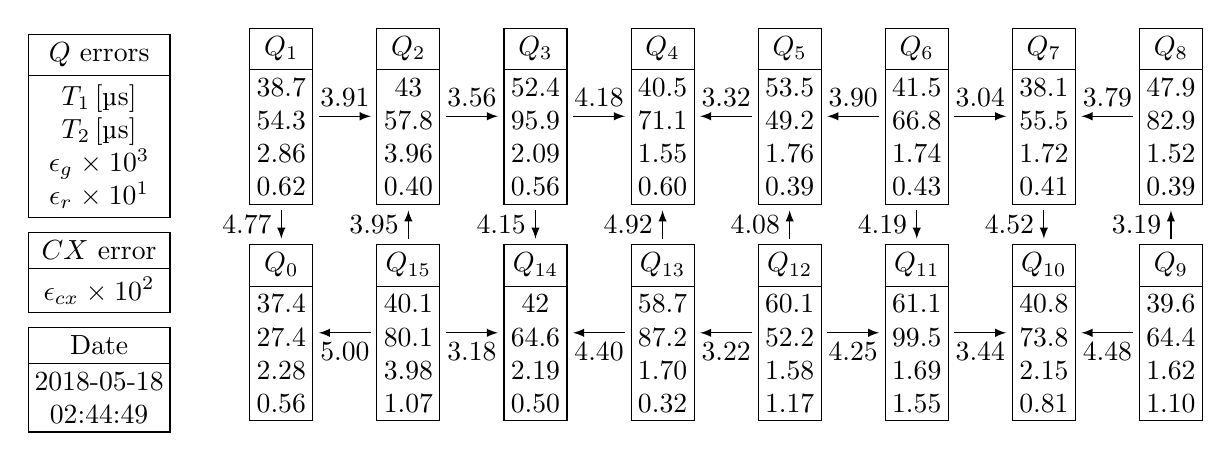
\begin{tikzpicture}[
block/.style={
    draw,
    fill=white,
    rectangle,
    inner xsep=0pt,
    inner ysep=\hp,
    text width=0.8cm,
    align=center,
},
myarrow/.style={
    -latex,
    shorten <= 2pt,
    shorten >= 2pt
}]

% {{{ qubits
\qubit{0}{37.4}{27.4}{2.28}{0.56};
\qubit{1}{38.7}{54.3}{2.86}{0.62};
\qubit{2}{43}{57.8}{3.96}{0.40};
\qubit{3}{52.4}{95.9}{2.09}{0.56};
\qubit{4}{40.5}{71.1}{1.55}{0.60};
\qubit{5}{53.5}{49.2}{1.76}{0.39};
\qubit{6}{41.5}{66.8}{1.74}{0.43};
\qubit{7}{38.1}{55.5}{1.72}{0.41};
\qubit{8}{47.9}{82.9}{1.52}{0.39};
\qubit{9}{39.6}{64.4}{1.62}{1.10};
\qubit{10}{40.8}{73.8}{2.15}{0.81};
\qubit{11}{61.1}{99.5}{1.69}{1.55};
\qubit{12}{60.1}{52.2}{1.58}{1.17};
\qubit{13}{58.7}{87.2}{1.70}{0.32};
\qubit{14}{42}{64.6}{2.19}{0.50};
\qubit{15}{40.1}{80.1}{3.98}{1.07};
% }}}
    \draw[myarrow] (Q1)  -- (Q2)  node[above, midway]{\displaycxerror{3.91}};
    \draw[myarrow] (Q1)  -- (Q0)  node[left , midway]{\displaycxerror{4.77}};
    \draw[myarrow] (Q2)  -- (Q3)  node[above, midway]{\displaycxerror{3.56}};
    \draw[myarrow] (Q3)  -- (Q4)  node[above, midway]{\displaycxerror{4.18}};
    \draw[myarrow] (Q3)  -- (Q14) node[left , midway]{\displaycxerror{4.15}};
    \draw[myarrow] (Q5)  -- (Q4)  node[above, midway]{\displaycxerror{3.32}};
    \draw[myarrow] (Q6)  -- (Q5)  node[above, midway]{\displaycxerror{3.90}};
    \draw[myarrow] (Q6)  -- (Q7)  node[above, midway]{\displaycxerror{3.04}};
    \draw[myarrow] (Q6)  -- (Q11) node[left , midway]{\displaycxerror{4.19}};
    \draw[myarrow] (Q7)  -- (Q10) node[left , midway]{\displaycxerror{4.52}};
    \draw[myarrow] (Q8)  -- (Q7)  node[above, midway]{\displaycxerror{3.79}};
    \draw[myarrow] (Q9)  -- (Q8)  node[left , midway]{\displaycxerror{3.19}};
    \draw[myarrow] (Q9)  -- (Q10) node[below, midway]{\displaycxerror{4.48}};
    \draw[myarrow] (Q11) -- (Q10) node[below, midway]{\displaycxerror{3.44}};
    \draw[myarrow] (Q12) -- (Q11) node[below, midway]{\displaycxerror{4.25}};
    \draw[myarrow] (Q12) -- (Q5)  node[left , midway]{\displaycxerror{4.08}};
    \draw[myarrow] (Q12) -- (Q13) node[below, midway]{\displaycxerror{3.22}};
    \draw[myarrow] (Q13) -- (Q14) node[below, midway]{\displaycxerror{4.40}};
    \draw[myarrow] (Q13) -- (Q4)  node[left , midway]{\displaycxerror{4.92}};
    \draw[myarrow] (Q15) -- (Q14) node[below, midway]{\displaycxerror{3.18}};
    \draw[myarrow] (Q15) -- (Q2)  node[left , midway]{\displaycxerror{3.95}};
    \draw[myarrow] (Q15) -- (Q0)  node[below, midway]{\displaycxerror{5.00}};


    \node(Qinfo) [block, text width=1.8cm, left=1cm of Q1, yshift=-0.12cm]{$Q$ errors\hsep $T_1\,[\si{\micro\second}]$\\ $T_2\,[\si{\micro\second}]$\\$\epsilon_g\times10^{3}$\\ $\epsilon_r\times10^{1}$  };
    \node(CXinfo)[block, text width=1.8cm, below=0.18cm of Qinfo] {$CX$ error \hsep $\epsilon_{cx}\times 10^{2}$};
    \node(Dateinfo) [block, text width=1.8cm, below=0.18cm of CXinfo] {Date \hsep 2018-05-18 \\ 02:44:49};

\end{tikzpicture}
\end{document}
